\chapter{Platform}
\label{chap:platform}

In chapter \ref{chap:intro}, I explained the motivations behind the
Custos. Chapter \ref{chap:purpose} outlines the design goals and
potential applications that these motivations suggest. In this
chapter, I'll discuss the architecture, interface, and implementation
of Custos platform.

\section{Architecture}

The Custos architecture contains several core components:

\begin{packed_item}
\item A standardized API and message exchange format promoting the
  creation and proliferation of multiple implementations across a
  selection of providers.
\item A flexible server-side authentication interface, supporting an
  extensible variety of authentication attributes.
\item A programable server-side access control system for associating
  authenticated attributes with key:value access rights on a per-key
  basis.
\item A server-side back-end key:value store for holding persistent
  user and implementation data
\item A server-side data system for storing and retrieving user data
\item A server-side auditing system for monitoring and recording
  key:value access and authentication attempt data.
\item A server-side management system for configuring and controlling
  the other components.
\item One or more client applications that offload encryption keys or
  other secrets to a Custos server for storage and access control.
\end{packed_item}

\begin{figure}[!tb]
  \vspace{5ex}
  \begin{center}
    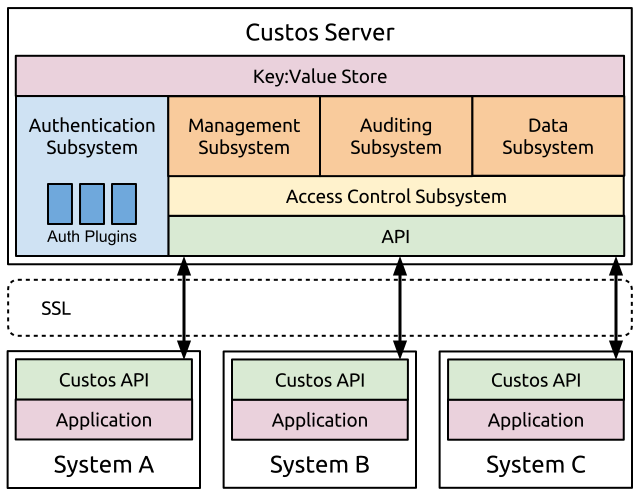
\includegraphics[width=.75\textwidth]
                    {./figs/pdf/Arch-Overview.pdf}
  \end{center}
  \caption{Basic Components of the Custos Architecture}
  \label{fig:arch-overview}
\end{figure}

Figure \ref{fig:arch-overview} shows the core Custos components. I'll
discuss the details of the Custos architecture in more details below.

\subsection{Overview}

The bulk of core Custos functionality is handled on the server
side. The server is designed to expose a single standardized API in
order to allow for a variety of inter-compatible implementations (one
possible implementation is discussed below). The Custos server
implements the following components:

\begin{packed_desc}
\item[API] \hfill \\ The server API handles all Custos requests,
  including requests for key:value data, requests to audit data
  access, and requests to modify data access controls. The API is
  essentially an RPC interface to allow applications to make requests
  of the Custos service.
\item[Access Control Subsystem] \hfill \\ The access control subsystem
  is the first step in the request processing pipeline after the
  API. The access control system compares the provided authentication
  attributes (calling into the authentication subsystem to verify
  them) to the set of required authentication attributes to determine
  if a Custos request should be allowed or denied.
\item[Authentication Subsystem] \hfill \\ The authentication
  subsystem's job is to verify the validity of any authentication
  attributes associated with a given Custos request. This subsystem is
  designed to allow for a pluggable authentication module interface
  capable of supporting a variety of authentication attributes.
\item[Data Subsystem] \hfill \\ The data subsystem is responsible for
  handling verified and accepted Custos data API requests (get, set,
  create, and delete key:value pairs). It interfaces with Key-Value
  store on one side and the access control system on the other.
\item[Auditing Subsystem] \hfill \\ The auditing subsystem is
  responsible for handling verified and accepted Custos audit API
  requests. The auditing subsystem is also concerned with logging all
  Custos requests and their corresponding responses. This data can
  then be used to generate reports related to the 'who', 'what', and
  'why' questions: \emph{Who} accessed (or failed to access)
  \emph{what} Custos stored data and \emph{why} where they granted or
  denied access (e.g. what authentication attributes did they present
  and were able to verify).
\item[Management Subsystem] \hfill \\ The management subsystem is
  responsible for handling all management related API requests after
  they have passed the authentication and access control layers. This
  primarily entails manipulating access control parameters.
\item[Key-Value Store] \hfill \\ The Key-Value store is the persistent
  data container associated with a given Custos server. It is used to
  store both end-user key:value pairs (encryption keys, etc) as well
  as a variety of internal Custos state (access control requirements,
  etc).
\end{packed_desc}

A Custos client applications interacts with a Custos server via the
API. As such, a client can simply offload the bulk of it's key
management directly to Custos through API-backed RPC libraries. Custos
simply becomes a remote key:value store where applications secrets are
stored. To satisfy Custos's authentication requirements, applications
can generate the necessary authentication attributes directly or can
instead pass these requirements on to the user, querying them for the
necessary attributes to send to Custos. Applications can either
implement their own auditing and management user controls directly,
passing the necessary information back to Custos via the API, or
applications can pass off auditing or management duties to separate
applications that interact directly with the Custos server.

\subsection{Access Control Abstraction}

As I already mentioned, the key:value abstraction Custos presents for
storing secrets is fairly well understood. It is Custos's access
control abstraction that is unique. This abstraction is at the core of
Custos's flexible capabilities.

The Custos abstraction control abstraction revolves around designating
an access control specification (ACS) for each object in the Custos
data store or for the Custos server itself. An ACS consists of three
components. First, each ACS contains a full list of the applicable
Custos \emph{permissions}. Associated with each permission is one or
more \emph{access control chains} (ACCs). Each ACC in turn consist of
an ordered list of \emph{authentication attributes}.

\subsubsection{Permissions}

The Custos access control model starts with the concepts of a
permission: a right to perform a specific Custos action. Custos
permissions are generally associated with the three core Custos
subsystems: data access, auditing, and access control. Custos also has
permission at two levels: per-server permissions, each associated with a
specific Custos server, and per-object permissions, each associated with
a specific key:value object.

The Custos data access permissions follow the pattern used by many
data access systems: permission to read data, permission to write
data, permission to create data, and permission to delete data. These
permissions are modified slightly to account for Custos's versioning
system. Unlike many system, Custos has no notion of object
ownership. Instead, it relies on priding access to each right an owner
would traditionally hold via explicit permissions. The per-server
Custos data access permissions are:

\begin{packed_desc}
\item[create] \hfill \\ The 'create' permission grants a user the
  right to create a new key:value object on a Custos server. When
  created, this object is associated with a programable default ACS
  similar to the Linux umask~\cite{man-umask} mechanism.
\end{packed_desc}

The per-object Custos data access permissions are:

\begin{packed_desc}
\item[delete] \hfill \\ The 'delete' permission grants a user the
  right to delete all versions of an existing key:value object.
\item[read] \hfill \\ The 'read' permission grants a user the right to
  read an exiting key:value object.
\item[update] \hfill \\ The 'update' permission grants a user the
  right to create a new version of a key:value object. It is the
  Custos equivalent of a ``write'' permission, but accounts for the fact
  the Custos key:value pairs are write-once objects, so ``writing'' to
  them really means creating a new version.
\end{packed_desc}

Similar to the data permissions, Custos associates audit permissions
with various entities. The per-server Custos audit permissions are:

\begin{packed_desc}
\item[audit-server] \hfill \\ The 'audit-server' permission grants a
  user the right to read all audit information not associated with an
  existing key:value object. This includes information related to
  requests for non-existent objects, object creation, etc.
\end{packed_desc}

The per-object Custos audit permissions are:

\begin{packed_desc}
\item[audit] \hfill \\ The 'audit' permission grants a user the right
  to read all audit information associated with an existing key:value
  object. This includes information related to object access (both
  granted and denied), object versioning, etc.
\item[clean] \hfill \\ The 'clean' permission grants a user the right
  to delete all audit information associated with an existing key:value
  object.
\end{packed_desc}

Finally, the Custos management permission control a users ability to
manage a Custos object or server. The per-server Custos management
permissions are:

\begin{packed_desc}
\item[mask-get] \hfill \\ The 'mask-get' permission grants a user the
  right to read the mask used to associate a default ACS with a newly
  created key:value pair.
\item[mask-set] \hfill \\ The 'mask-set' permission grants a user the
  right to set the mask used to associate a default ACS with a newly
  created key:value pair.
\end{packed_desc}

The per-object Custos management permissions are:

\begin{packed_desc}
\item[acs-get] \hfill \\ The 'acs-get' permission grants a user the
  right to view the ACS associated with an existing key-value pair.
\item[acs-set] \hfill \\ The 'acs-set' permission grants a user the
  right to set the ACS associated with an existing key-value pair.
\end{packed_desc}

\subsubsection{Access Control Chains}


\subsubsection{Authentication Attributes}


\section{Interface}

\subsection{Data API Components}

For getting, setting keys

\subsection{Management API Components}

For controlling keys

\subsection{Auditing API Components}

For auditing  keys

\section{Implementation}

\subsection{API}

JSON RESTful API

\subsection{Authentication and Access Control}

Standardized module interface

\subsection{Back-end Storage}

Variable back-end key-value providers

%%  LocalWords:  ACS ACCs ACC acs
